\documentclass[12pt, a4paper]{article}

\usepackage{ctex}
\usepackage{float, booktabs, parskip}
\usepackage{amsmath, amsthm, amssymb, mathrsfs, bm}
\usepackage{graphicx, subfigure, svg}
\usepackage{algorithm, algorithmicx, algpseudocode}
\usepackage{hyperref, endnotes}

\setlength{\parindent}{4em}
\setlength{\parskip}{1em}
\allowdisplaybreaks[4]

\newcommand{\under}[1]{\mathop{#1}\limits_}
\newcommand{\vv}[1]{{\bm{#1}}}

\newcommand{\al}{{\overline{\alpha}}}
\newcommand{\HH}{{\mathcal{H}}}
\newcommand{\EE}{{\mathcal{E}}}
\newcommand{\prob}{{\mathbb{P}}}
\newcommand{\unit}{{\mathbb{I}}}
\newcommand{\st}{{\text{s.t.}}}


\title{{\Huge{\textbf{Report on Homework 3 \\}}} —— Machine Learning}
\author{刘滨瑞 \\ 2021012579 \quad 未央-水木12}

\begin{document}

\maketitle

\stepcounter{section}

\section{决策树与随机森林}

    \subsection{ID3算法无法找到最优解的一个情形}

        \begin{enumerate}

        \item 证明：使用ID3算法得到的决策树至少有$\frac{1}{4}$的训练误差。

            第一次分割：

            若按1号特征分割，信息增益为：
            \begin{align*}
            IG = (-\frac{2}{4} \log_2 \frac{2}{4} - \frac{2}{4} \log_2 \frac{2}{4}) - \frac{3}{4} (-\frac{2}{3} \log_2 \frac{2}{3} -\frac{1}{3} \log_2 \frac{1}{3}) - 0 = 0.311
            \end{align*}
            若按2号特征或3号特征分割，信息增益为：
            \begin{align*}
            IG = (-\frac{2}{4} \log_2 \frac{2}{4} - \frac{2}{4} \log_2 \frac{2}{4}) - 2 \times \frac{2}{4} (-\frac{1}{2} \log_2 \frac{1}{2} -\frac{1}{2} \log_2 \frac{1}{2}) = 0
            \end{align*}

            因此，在ID3算法中，第一次分割应基于1号特征。此时，决策树形状如图1所示。
            右侧子集合已完成分类，在第二次分割时，我们只需要关注左侧子集合。

            \begin{figure}[htbp]
            \centering
            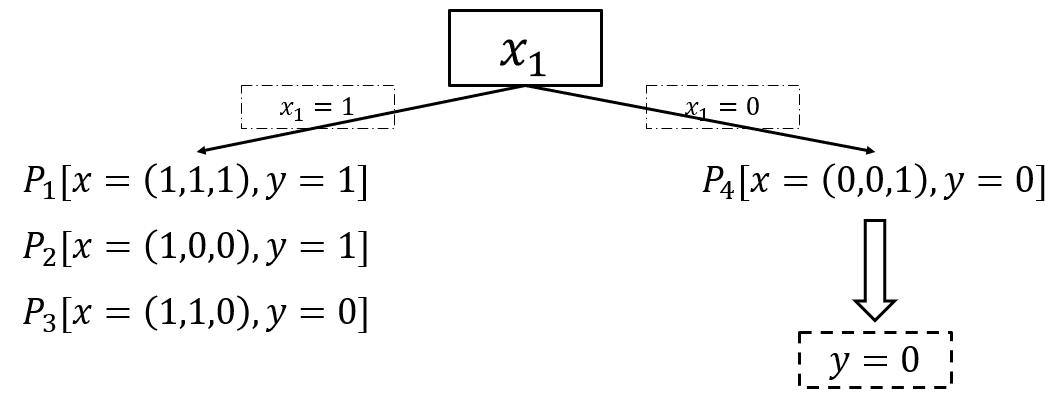
\includegraphics[width=0.90\textwidth]{./assets/DT_1.png}
            \caption{第一次分割后的决策树形状}
            \end{figure}

            第二次分割：

            无论按照2号特征还是3号特征，信息增益均为：
            \begin{align*}
            IG = (-\frac{2}{3} \log_2 \frac{2}{3} - \frac{1}{3} \log_2 \frac{1}{3}) - \frac{2}{3} (-\frac{1}{2} \log_2 \frac{1}{2} -\frac{1}{2} \log_2 \frac{1}{2}) - 0 = 0.252
            \end{align*}

            因此，在ID3算法中，第二次分割等可能地基于2号特征或3号特征。此时，可能的决策树形状如图2所示。

            \begin{figure}[htbp]
            \centering
            \subfigure[基于2号特征进行分割]{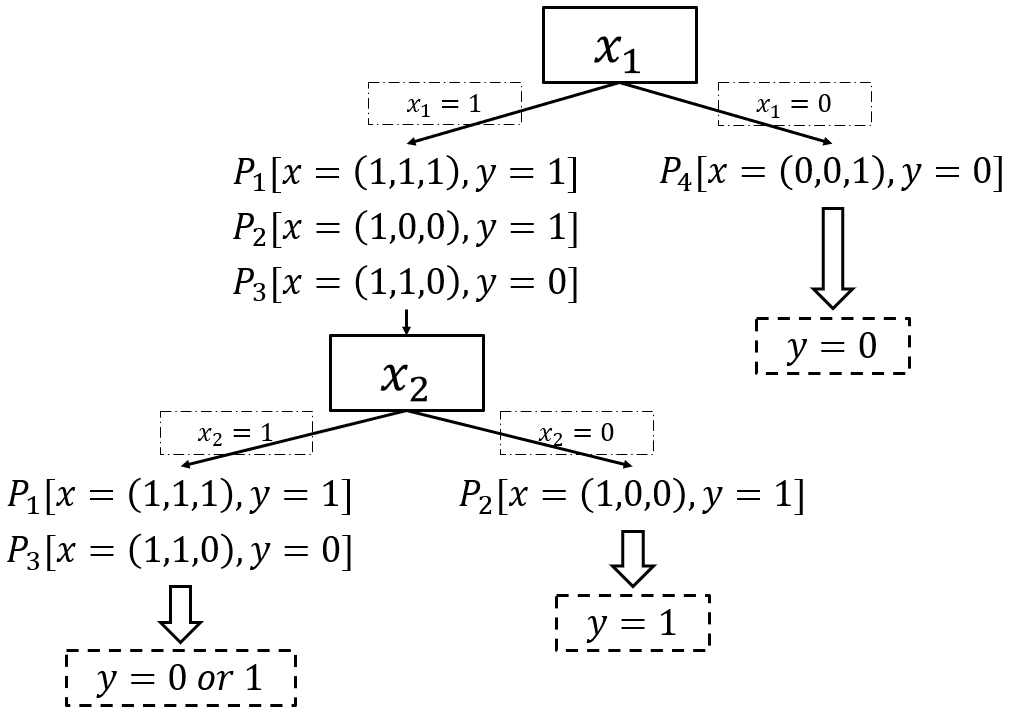
\includegraphics[width=0.48\textwidth]{./assets/DT_2.png}}
            \subfigure[基于3号特征进行分割]{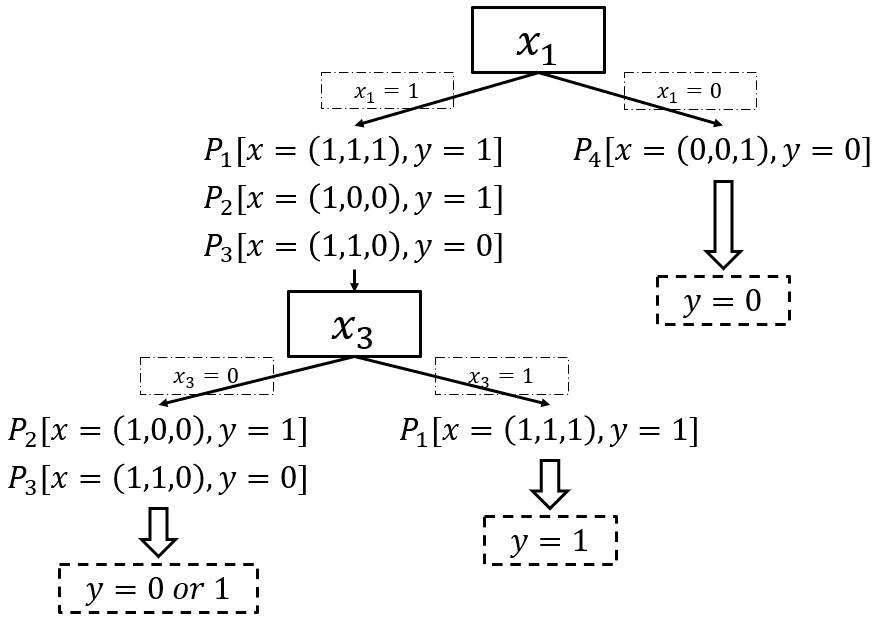
\includegraphics[width=0.48\textwidth]{./assets/DT_3.png}}
            \caption{第二次分割后的决策树形状}
            \end{figure}

            可以看出，在两种深度为2的决策树中，均存在一个叶节点含有两种类别的样本，因此至少有一个样本会被错误分类。
            这即说明了基于ID3算法得到的决策树至少会有$\frac{1}{4}$的训练误差。

        \item 构造一棵深度为$2$，且训练误差为$0$的决策树。

            图3所示的决策树满足题目要求。

            \begin{figure}[htbp]
            \centering
            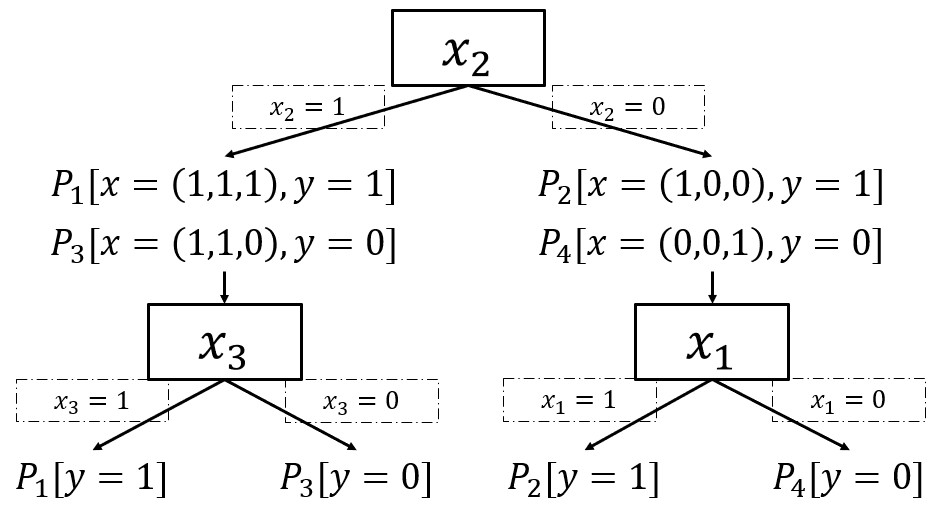
\includegraphics[width=0.90\textwidth]{./assets/DT_4.png}
            \caption{深度为2，训练误差为0的决策树}
            \end{figure}

        \end{enumerate}

    \subsection{随机森林}

        \begin{enumerate}

        \item 求任意一个特定的特征从未被选中分割的概率。

            考虑到随机森林中的每棵二叉决策树都有$h$个内部节点，
            而每个节点都会从本树未使用过的特征中随机选取$K = 1$个用于分类决策。
            因此，选取特征的过程等价于：每棵决策树随机地从$d$个特征中选取$h$个。
            故对于某一特定的特征，任意一棵决策树中未使用此特征的概率为：$1 - \frac{h}{d}$。

            由于每个决策树选取特征的过程相互独立，在总共$t$棵决策树中，
            任意一个特定的特征从未被选中分割的概率为：
            \begin{align*}
            \prob = (1 - \frac{h}{d})^t
            \end{align*}

        \item 求任意一个特定的样本从未在任何一棵树中被考虑的概率。

            每棵决策树会使用$m$个自主采样得到的样本，总样本规模为$n$。
            对于某一特定的样本，在任意一棵决策树中未考虑过该样本的概率为：$(1 - \frac{1}{n})^m$。

            同样地，由于每个决策树采样的过程相互独立，在总共$t$棵决策树中，
            任意一个特定的样本从未在任何一棵树中被考虑的概率为：
            \begin{align*}
            \prob = (1 - \frac{1}{n})^{mt}
            \end{align*}

        \end{enumerate}

    \subsection{代码实验}

        决策树的实现代码已经按要求补全，详见./code/tree.py中的相应部分。

        决策树在二分类问题和回归问题上的结果如图4、图5所示。

        \begin{figure}[htbp]
        \centering
        
\includegraphics[width=0.96\textwidth]{./assets/DT_entropy.pdf}
        \caption{决策树在二分类问题上的结果}
        \end{figure}

        \begin{figure}[htbp]
        \centering
        
\includegraphics[width=0.96\textwidth]{./assets/DT_regression.pdf}
        \caption{决策树在回归问题上的结果}
        \end{figure}

        \begin{figure}[htbp]
        \centering
        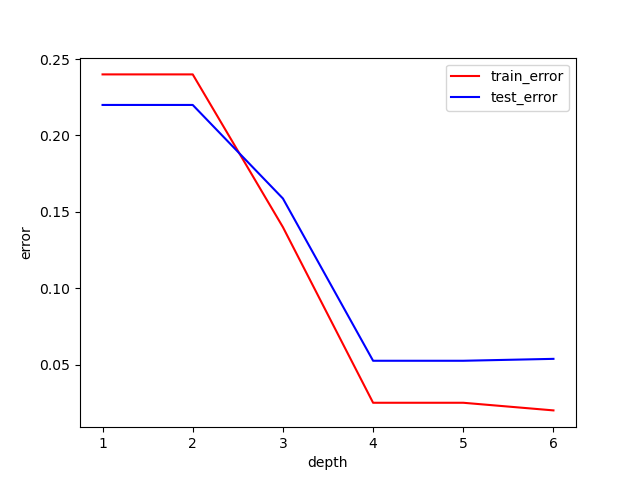
\includegraphics[width=0.80\textwidth]{./assets/DT_0c.png}
        \caption{在二分类问题上，不同深度的决策树的训练误差与测试误差}
        \end{figure}

        \begin{figure}[htbp]
        \centering
        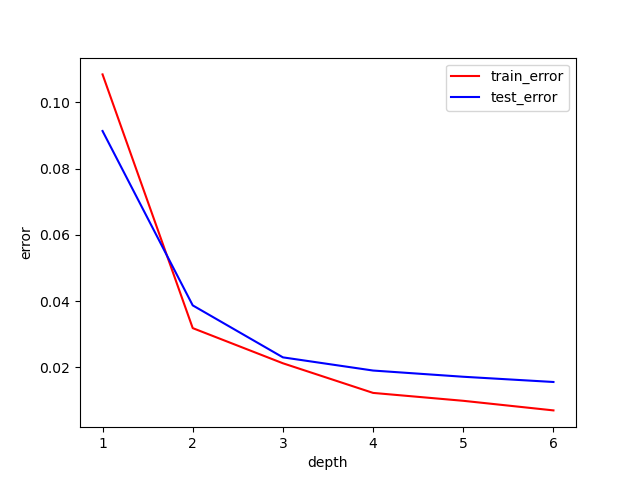
\includegraphics[width=0.80\textwidth]{./assets/DT_0r.png}
        \caption{在回归问题上，不同深度的决策树的训练误差与测试误差}
        \end{figure}

        另外，在两类问题中，我们还统计了不同深度的决策树的训练误差和测试误差。
        将结果绘制成图像，如图6、图7所示。

        可以看出，决策树在训练集中的误差随着深度的提高而迅速下降，拟合数据的能力明显提高。
        这是因为决策树的深度越大，其就拥有更多可用于分类判断的子节点，
        从而使得模型具有更高的复杂度与拟合能力，可以捕捉到更多数据中的特征。

        在二分类问题中，当决策树深度大于$4$后，模型在测试集上的误差已经不再继续降低，体现出的分类效果也已经十分良好，
        这说明取决策树深度等于$4$是较为合适的，模型在该深度下可以充分拟合数据。
        此时如果继续提高决策树的深度，可能会出现过拟合的问题。

        而在回归问题中，直到深度等于$6$时，模型在测试集上的误差仍保持着继续降低的趋势，
        此时可以进一步提高决策树的深度，以更好地拟合数据。

\section{提升算法}

    \subsection{噪声不敏感的AdaBoost算法}

        \begin{enumerate}

        \item 证明$G$是$\mathbb{R}$上的凸函数且处处可导。

            显然，在$(-\infty, 0]$和$[0, \infty)$上，$G$均为可导的凸函数。
            我们只需要证明$G$在$0$处的左右导数相等，
            并证明对于任意的$x_1 \le 0, x_2 > 0$和$\lambda \in (0, 1)$，
            有$\lambda G(x_1) + (1 - \lambda) G(x_2) \ge G(\lambda x_1 + (1 - \lambda) x_2)$成立即可。

            对于第一个子命题，有：
            \begin{align*}
            G^\prime(x) \vert_{x = 0^-} =& (e^x) \vert_{x = 0^-} = 1 \\
            G^\prime(x) \vert_{x = 0^+} =& (1) \vert_{x = 0^+} = 1
            \end{align*}
            二者相等，子命题成立。

            对于第二个子命题，若$x_0 = \lambda x_1 + (1 - \lambda) x_2 > 0$，则：
            \begin{align*}
            \lambda G(x_1) + (1 - \lambda) G(x_2)
            =& \lambda e^{x_1} + (1 - \lambda) (x_2 + 1) \\
            \ge& \lambda (x_1 + 1) + (1 - \lambda) (x_2 + 1) \\
            =& (\lambda x_1 + (1 - \lambda) x_2) + 1 = G(x_0)
            \end{align*}
            若$x_0 \le 0$，此时有$\lambda \ge \frac{x_0}{x_1}$。
            我们构造函数$u(x) = \frac{e^{x} - 1}{x}, x \le 0$。使用常用不等式$e^x \le \frac{1}{1 - x}$：
            \begin{align*}
            u^\prime(x) = \frac{x e^x - e^x + 1}{x^2} \ge \frac{(x - 1)(\frac{1}{1 - x}) + 1}{x^2} = 0
            \end{align*}
            这说明$u(x)$是递增函数，于是：
            \begin{align*}
            \lambda G(x_1) + (1 - \lambda) G(x_2) - G(x_0)
            =& \lambda e^{x_1} + (1 - \lambda) (\frac{x_0 - \lambda x_1}{1 - \lambda} + 1) - e^{x_0} \\
            =& \lambda e^{x_1} + x_0 - \lambda x_1 + 1 - \lambda - e^{x_0} \\
            =& \lambda (e^{x_1} - x_1 - 1) - (e^{x_0} - x_0 - 1) \\
            \ge& x_0 (\frac{e^{x_1} - x_1 - 1}{x_1} - \frac{e^{x_0} - x_0 - 1}{x_0}) \\
            =& -x_0 (u(x_0) - u(x_1)) \ge 0
            \end{align*}
            即：$\lambda G(x_1) + (1 - \lambda) G(x_2) \ge G(x_0)$，子命题成立。

            综上，我们证明了$G$是$\mathbb{R}$上处处可导的凸函数。

        \item 给出第$t$步时弱分类器$h_t$应当优化的损失函数$\epsilon_t$的表达式。

            在第$t$步时，待优化的损失函数$\epsilon_t$可表示为：
            \begin{align*}
            \epsilon_t = \sum_{i = 1}^{m} \overline{D}_t(i) \unit_{[y_i \ne h_t(\vv{x}_i)]}
            \end{align*}
            下面，我们给出$\overline{D}_t(i)$的表达式。

            设$\HH = \{h_1, h_2, ..., h_N\}$，第$t$步时，若在方向$k$上执行坐标下降，有：
            \begin{align*}
            &F^\prime(\vv{\al}_{t - 1}, \vv{e}_k) \\
            =& \lim_{\eta \rightarrow 0} \frac{F(\vv{\al}_{t - 1} + \eta \vv{e}_k) - F(\vv{\al}_{t - 1})}{\eta} \\
            =& \lim_{\eta \rightarrow 0} \frac{1}{\eta} (\frac{1}{m} \sum_{i = 1}^{m} (G(-y_i \vv{\al}_{t - 1}^T \vv{h}(\vv{x}_i) - \eta y_i h_k(\vv{x}_i)) - G(-y_i \vv{\al}_{t - 1}^T \vv{h}(\vv{x}_i)))) \\
            =& -\frac{1}{m} \sum_{i = 1}^{m} y_i h_k(\vv{x}_i) G^\prime(-y_i \sum_{j = 1}^{N} \al_{t - 1, j} h_j(\vv{x}_i))
            \end{align*}

            按AdaBoost算法的定义，此时应满足：
            \begin{align*}
            \overline{D}_t(i) \overline{Z}_t = G^\prime(-y_i \sum_{j = 1}^{N} \al_{t - 1, j} h_j(\vv{x}_i))
            \end{align*}
            其中$\overline{Z}_t$为归一化因子，$G^\prime$由3.1.1中求得的导数定义。

            综上，我们有：
            \begin{align*}
            \overline{Z}_t =& \sum_{i = 1}^{m} G^\prime(-y_i \sum_{j = 1}^{N} \al_{t - 1, j} h_j(\vv{x}_i)) \\
            \overline{D}_t(i) =& \frac{G^\prime(-y_i \sum_{j = 1}^{N} \al_{t - 1, j} h_j(\vv{x}_i))}{\overline{Z}_t}
            \end{align*}

        \end{enumerate}

    \subsection{探究AdaBoost算法是否能使用完全相同的弱分类器}

        \begin{enumerate}

        \item 证明：$\sum_{i = 1}^{m} D_{t + 1}(i) \unit_{[y_i \ne h_t(\vv{x}_i)]} = \frac{1}{2}$。

            首先，注意到：
            \begin{align*}
            \sum_{i = 1}^{m} D_{t + 1}(i) \unit_{[y_i \ne h_t(\vv{x}_i)]} + \sum_{i = 1}^{m} D_{t + 1}(i) \unit_{[y_i = h_t(\vv{x}_i)]} = \sum_{i = 1}^{m} D_{t + 1}(i) = 1
            \end{align*}
            因此，只需要证明：
            \begin{align*}
            \sum_{i = 1}^{m} D_{t + 1}(i) \unit_{[y_i \ne h_t(\vv{x}_i)]} = \sum_{i = 1}^{m} D_{t + 1}(i) \unit_{[y_i = h_t(\vv{x}_i)]}
            \end{align*}

            我们有：
            \begin{align*}
            &\sum_{i = 1}^{m} D_{t + 1}(i) \unit_{[y_i \ne h_t(\vv{x}_i)]} - \sum_{i = 1}^{m} D_{t + 1}(i) \unit_{[y_i = h_t(\vv{x}_i)]} \\
            =& \frac{1}{Z_t} (\sum_{i = 1}^{m} e^{-\alpha_t y_i h_t(\vv{x}_i)} D_{t}(i) \unit_{[y_i \ne h_t(\vv{x}_i)]} - \sum_{i = 1}^{m} e^{-\alpha_t y_i h_t(\vv{x}_i)} D_{t}(i) \unit_{[y_i = h_t(\vv{x}_i)]}) \\
            =& \frac{1}{Z_t} (\sum_{i, y_i \ne h_t(\vv{x}_i)} e^{\alpha_t} D_{t}(i) - \sum_{i, y_i = h_t(\vv{x}_i)} e^{-\alpha_t} D_{t}(i)) \\
            =& \frac{1}{Z_t} (\sum_{i, y_i \ne h_t(\vv{x}_i)} e^{\frac{1}{2} \log \frac{1 - \epsilon_t}{\epsilon_t}} D_{t}(i) - \sum_{i, y_i = h_t(\vv{x}_i)} e^{-\frac{1}{2} \log \frac{1 - \epsilon_t}{\epsilon_t}} D_{t}(i)) \\
            =& \frac{1}{Z_t} (\sqrt{\frac{1 - \epsilon_t}{\epsilon_t}} \sum_{i, y_i \ne h_t(\vv{x}_i)} D_{t}(i) - \sqrt{\frac{\epsilon_t}{1 - \epsilon_t}} \sum_{i, y_i = h_t(\vv{x}_i)} D_{t}(i)) \\
            =& \frac{1}{Z_t} (\sqrt{\frac{1 - \epsilon_t}{\epsilon_t}} (\epsilon_t) - \sqrt{\frac{\epsilon_t}{1 - \epsilon_t}} (1 - \epsilon_t)) \\
            =& 0
            \end{align*}
            命题得证。

        \item 说明第$t + 1$步选取的弱分类器$h_{t + 1}$不会与$h_t$相同。

            若第$t + 1$步选取的弱分类器$h_{t + 1} = h_t$，则：
            \begin{align*}
            \epsilon_{t + 1} = \sum_{i = 1}^{m} D_{t + 1} \unit_{[y_i \ne h_{t + 1}(\vv{x}_i)]} = \sum_{i = 1}^{m} D_{t + 1} \unit_{[y_i \ne h_t(\vv{x}_i)]} = \frac{1}{2}
            \end{align*}

            但是，在AdaBoost算法中，我们选取的$h_{t + 1}$是在$t + 1$轮迭代中具有最小经验误差的合法弱分类器，
            必然有$\epsilon_{t + 1} < \frac{1}{2}$成立，矛盾！

            因此，第$t + 1$步选取的弱分类器$h_{t + 1}$不会与$h_t$相同。

        \end{enumerate}

    \subsection{AdaBoost的训练误差}

        \begin{enumerate}

        \item 证明：当$T > \frac{\log m}{2 \gamma^2}$时，AdaBoost的训练误差可以达到$0$。

            根据课件上的结论，AdaBoost算法的训练误差存在一个上界：
            \begin{align*}
            \hat{\EE}(h) \le \exp(-2 \gamma^2 T) < \exp(-2 \gamma^2 \frac{\log m}{2 \gamma^2}) = \frac{1}{m}
            \end{align*}

            另一方面，若$\hat{\EE}(h) > 0$，则意味着至少有一个样本被错误分类。根据$\hat{\EE}(h)$的定义：
            \begin{align*}
            \hat{\EE}(h) = \frac{1}{m} \sum_{i = 1}^{m} \unit_{[y_i f(\vv{x}_i) \le 0]} \ge \frac{1}{m}
            \end{align*}
            矛盾！因此，当$T > \frac{\log m}{2 \gamma^2}$时，有$\hat{\EE}(h) = 0$成立。

        \end{enumerate}

    \subsection{简化版本的AdaBoost}

        \begin{enumerate}

        \item 试找出一个合理的固定$\alpha$取值，使得最终得到的分类器的训练误差不多于$(1 - 4 \gamma^2)^{\frac{T}{2}}$。

            取$\alpha = \frac{1}{2} \log \frac{1 + 2 \gamma}{1 - 2 \gamma}$，
            下面我们证明AdaBoost算法训练得到的分类器的训练误差不多于$(1 - 4 \gamma^2)^{\frac{T}{2}}$。

            根据训练误差的定义：
            \begin{align*}
            \hat{\EE}(h) = \frac{1}{m} \sum_{i = 1}^{m} \unit_{[y_i f(\vv{x}_i) \le 0]}
            \le& \frac{1}{m} \sum_{i = 1}^{m} e^{-y_i f(\vv{x}_i)} \\
            \le& \frac{1}{m} \sum_{i = 1}^{m} (m \prod_{t = 1}^{T} Z_t) D_{T + 1}(i) \\
            =& \prod_{t = 1}^{T} Z_t
            \end{align*}
            而对于每个$Z_t$，有：
            \begin{align*}
            Z_t = \sum_{i = 1}^{m} D_t(i) e^{-\alpha y_i h_t(\vv{x}_i)}
            =& \sum_{i, y_i \ne h_t(\vv{x}_i)} e^{\alpha} D_{t}(i) + \sum_{i, y_i = h_t(\vv{x}_i)} e^{-\alpha} D_{t}(i) \\
            =& \epsilon_t e^{\alpha} + (1 - \epsilon_t) e^{-\alpha} \\
            =& \epsilon_t \sqrt{\frac{1 + 2 \gamma}{1 - 2 \gamma}} + (1 - \epsilon_t) \sqrt{\frac{1 - 2 \gamma}{1 + 2 \gamma}} \\
            \le& \frac{1 - 2 \gamma}{2} \sqrt{\frac{1 + 2 \gamma}{1 - 2 \gamma}} + \frac{1 + 2 \gamma}{2} \sqrt{\frac{1 - 2 \gamma}{1 + 2 \gamma}} \\
            =& \frac{1}{2} \sqrt{1 - 4 \gamma^2} + \frac{1}{2} \sqrt{1 - 4 \gamma^2} \\
            =& \sqrt{1 - 4 \gamma^2}
            \end{align*}

            综上，
            \begin{align*}
            \hat{\EE}(h) = \prod_{t = 1}^{T} Z_t \le (\sqrt{1 - 4 \gamma^2})^T = (1 - 4 \gamma^2)^{\frac{T}{2}}
            \end{align*}

        \end{enumerate}

    \subsection{Gradient Boosting Machines}

        \begin{enumerate}

        \item 算法流程补全。

            (b) $h_t = \under{\arg\min}{h \in \mathcal{F}} \sum_{i = 1}^{n} (h(\vv{x}_i) + \vv{g}_{t, i})^2$

            (d) $f_t(\vv{x}) = f_{t - 1}(\vv{x}) + \alpha_t h_t(\vv{x})$

        \item 回归问题中的$\vv{g}_t$与$h_t$。

            将损失函数的形式代入3.5.1中，得：
            \begin{align*}
            \vv{g}_t =& (\hat{\vv{y}}_i - \vv{y}_i)_{i = 1}^{n} = (f_{t - 1}(\vv{x}_i) - \vv{y}_i)_{i = 1}^{n} \\
            h_t =& \under{\arg\min}{h \in \mathcal{F}} \sum_{i = 1}^{n} (h(\vv{x}_i) + f_{t - 1}(\vv{x}_i) - \vv{y}_i)^2
            \end{align*}

        \item 二分类问题中的$\vv{g}_t$与$h_t$。

            将损失函数的形式代入3.5.1中，得：
            \begin{align*}
            \vv{g}_t =& (\frac{-\vv{y}_i}{1 + e^{\vv{y}_i \hat{\vv{y}}_i}})_{i = 1}^{n} = (\frac{-\vv{y}_i}{1 + e^{\vv{y}_i f_{t - 1}(\vv{x}_i)}})_{i = 1}^{n} \\
            h_t =& \under{\arg\min}{h \in \mathcal{F}} \sum_{i = 1}^{n} (h(\vv{x}_i) - \frac{\vv{y}_i}{1 + e^{\vv{y}_i f_{t - 1}(\vv{x}_i)}})^2
            \end{align*}

        \item 代码实验。

            GBM的实现代码已经按要求补全，详见./code/boosting.py中的相应部分。

            使用L2 loss的GBM在二分类问题和回归问题上的结果如图8、图10所示。

            使用logistics loss的GBM在二分类问题上的结果如图9所示。

            \begin{figure}[htbp]
            \centering
            
\includegraphics[width=0.80\textwidth]{./assets/GBM_l2.pdf}
            \caption{使用L2 loss的GBM在二分类问题上的结果}
            \end{figure}

            \begin{figure}[htbp]
            \centering
            
\includegraphics[width=0.80\textwidth]{./assets/GBM_logistic.pdf}
            \caption{使用logistics loss的GBM在二分类问题上的结果}
            \end{figure}

            \begin{figure}[htbp]
            \centering
            
\includegraphics[width=0.96\textwidth]{./assets/GBM_regression.pdf}
            \caption{使用L2 loss的GBM在回归问题上的结果}
            \end{figure}

            \begin{figure}[htbp]
            \centering
            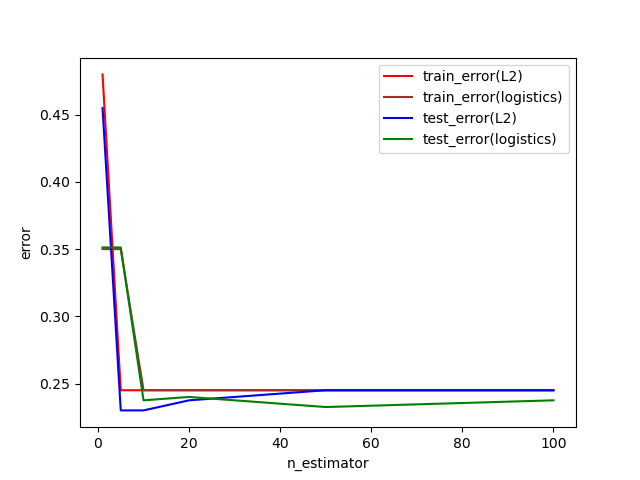
\includegraphics[width=0.88\textwidth]{./assets/GBM_0c.png}
            \caption{在二分类问题上，不同基学习器数目GBM的训练误差与测试误差}
            \end{figure}

            \begin{figure}[htbp]
            \centering
            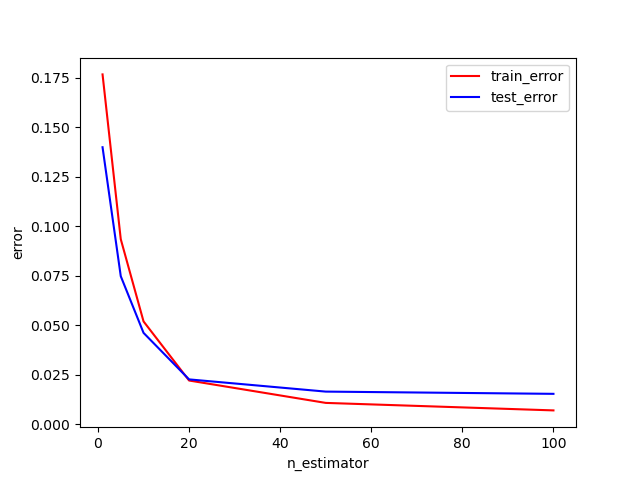
\includegraphics[width=0.88\textwidth]{./assets/GBM_0r.png}
            \caption{在回归问题上，不同基学习器数目GBM的训练误差与测试误差}
            \end{figure}

            另外，在两类问题中，我们还统计了不同基学习器数目情况下模型的训练误差和测试误差。
            将结果绘制成图像，如图11、图12所示。

            可以看出，在二分类问题中，不论使用哪一种损失函数，GBM在训练集上的误差都随着基学习器数目的增加而极快地降低，
            在$n_{estimator} > 10$时，GBM在训练集上的误差已完全收敛，在结果中也表现出了优秀的分类效果。
            这印证了课堂上我们基于学习理论得出的结论：GBM有着非常强的拟合能力。

            而当$n_{estimator}$在$10$左右时，GBM在验证集上的误差已达到最小值，
            此后若继续提高$n_{estimator}$，在验证集上的误差反而增大。
            这说明在$n_{estimator} > 10$时，模型出现了过拟合问题。

            横向对比L2损失函数与logistics损失函数，两种GBM在训练集与测试集上的最小损失相近，
            但基于logistics损失函数的GBM收敛更慢，推测可能的原因是：logistics损失函数的梯度信号更弱。

            而在回归问题中，随着基学习器数目的增多，模型在训练集和测试集上的误差仍保持着继续降低的趋势，
            说明即使在$n_{estimator} = 100$时，我们仍可以继续增加基学习器的数目以获得更好的模型性能。

        \end{enumerate}

\end{document}
